\documentclass[11pt]{article}
\usepackage[margin=0.85in]{geometry}
\usepackage[T1]{fontenc}
\usepackage{lmodern}
\usepackage{amsmath,amssymb,booktabs,longtable,array,tabularx}
\usepackage[dvipsnames]{xcolor}
\usepackage{enumitem}
\usepackage{microtype}
\usepackage{tikz}
\usetikzlibrary{arrows.meta,positioning}
\usepackage[colorlinks=true,linkcolor=MidnightBlue,urlcolor=MidnightBlue,citecolor=MidnightBlue]{hyperref}
\urlstyle{same}
\setlength{\parindent}{0pt}
\setlength{\parskip}{6pt}
\setlist{nosep,leftmargin=*}
\newcolumntype{P}[1]{>{\raggedright\arraybackslash}p{#1}}
\title{Interaction for the Digital Professor\\\large Reference Notes and Prototype Concept}
\author{Jonathan Ma}
\date{\today}

\begin{document}
\maketitle

\section{Scope}
This project aims to create a course-agnostic digital professor or teaching assistant. These notes examine its \emph{interaction layer}: how students ask questions, share their work, and receive feedback. Statistics and engineering provide demanding initial examples because explanations frequently combine prose, equations, plots, and intermediate solution steps. Multimodal generative AI can connect these representations, but interface capability alone does not establish teaching competence or AGI.

\textbf{Recommended initial experience:} A chatbot-style web application with three tabs: Sources, Provider Settings, and Chat. On first use, the app prompts the student to upload a syllabus, extracts a proposed course name and basic course metadata, and asks the student to confirm or edit them. Students can then attach documents, images, equations, handwriting, or recorded speech and ask open-ended questions. One tutoring orchestrator identifies the student's intent and calls deterministic modality services. A visible \emph{Office Hours} option communicates the longer-term direction, but synchronous office-hours tutoring is marked \emph{Coming Soon} during the initial prototype.

Assume a small student team, ordinary laptops/tablets, internet access, modest paid API use, and no model training or dedicated GPU requirement. Exact prices, account availability, model identifiers, and preview status will be checked when implementation begins. 

\part{Existing and Emerging Interaction Methods}

\section{Comparison at a glance}
Define implementation feasibility on three levesls: high, medium, and lower. High indicates reuse of standard interfaces or hosted services, medium indicates we'll need to tune input integration, and low means we may need to build from the ground up.  Effort is relative engineering effort, not a time estimate. Cloud services introduce usage charges and data transfer; locally runnable libraries introduce maintenance and hardware costs.

\small
\begin{longtable}{@{}P{0.15\textwidth}P{0.28\textwidth}P{0.32\textwidth}P{0.17\textwidth}@{}}
\toprule
Dimension & Candidate technologies & Value and principal constraint & Initial feasibility \\
\midrule
\endfirsthead
\toprule Dimension & Candidate technologies & Value and principal constraint & Initial feasibility \\
\midrule
\endhead
Text & Responses API; browser chat; KaTeX \cite{text,katex} & Precise, searchable dialogue; generated explanations still need grounding and checking. & High; low effort. Core. \\
\addlinespace
Voice conversation & OpenAI Realtime; Gemini Live; LiveKit Agents \cite{realtime,live,livekit} & Natural follow-ups and interruptions; turn detection, reconnects, and shared visual context add work. & Medium; medium--high effort. Later. \\
\addlinespace
Speech recognition / response & MediaRecorder; hosted transcription and TTS; faster-whisper; Web Speech API \cite{recorder,stt,tts,whisper,webspeech} & Spoken questions and read-aloud hints; symbols, accents, noise, and playback require testing. & High for push-to-talk; low--medium effort. Optional early. \\
\addlinespace
Long-form audio & File transcription; timestamped segments; persistent session notes \cite{stt,whisper} & Review an explanation or resume tutoring; chunking and summaries can lose details. & High for bounded recordings; medium effort. After core. \\
\addlinespace
Documents & PDF.js; direct file input; Docling; hosted file search \cite{pdfjs,files,docling,retrieval} & Discuss notes and student work; reading order, scans, and citation accuracy vary. & High for selected pages; medium effort. Core. \\
\addlinespace
Handwriting / stylus & Pointer Events + canvas; MyScript iinkTS; Mathpix \cite{pointer,myscript,mathpix} & Preserve derivations and sketches; ink capture is easier than reliable interpretation. & High for snapshots, medium for recognition. Early extension. \\
\addlinespace
Mathematical expressions & MathLive; KaTeX; Mathpix; SymPy \cite{mathlive,katex,mathpix,sympy} & Structured input, display, and bounded checking; notation and assumptions remain ambiguous. & High for entry/display; medium for checking. Core. \\
\addlinespace
Image / camera & File upload; getUserMedia; vision model; Mathpix \cite{media,vision,mathpix} & Share paper, plots, or diagrams; tiny labels and spatial reasoning can fail. & High for still images; low--medium effort. Core. \\
\addlinespace
Tablet / iPad & Responsive web UI; Pointer Events; native PencilKit \cite{pointer,pencil} & Read, write, and discuss together; touch, keyboard, palm handling, and browser behavior need device testing. & High for web access; medium for polished pen UX. Core web. \\
\addlinespace
Video & Gemini video understanding; Gemini Live; MediaRecorder \cite{video,live,recorder} & Explain an evolving procedure; sampling, bandwidth, and temporal alignment complicate feedback. & Medium for clips; lower for continuous tutoring. Later. \\
\bottomrule
\end{longtable}
\normalsize

\section{Detailed technology notes}
Each modality below is treated as a capability attached to the same chatbot conversation. The student asks a question in chat; the tutoring orchestrator identifies the intent, selects relevant sources and tools, and returns one coherent response.

\subsection{Text-based interaction}
\begin{itemize}
\item \textbf{Role in the chatbot:} The interaction default. Students ask open-ended questions, revise them, inspect prior feedback, and select actions such as \emph{Hint}, \emph{Explain}, \emph{Check my work}, or \emph{Quiz me}.
\item \textbf{Technologies:} a hosted model through an API such as OpenAI Responses, streaming chat UI, conversation storage, and KaTeX for equation rendering.\cite{text,katex}
\item \textbf{Context handling:} send the current message, recent dialogue, selected course sources, and student artifacts to the tutoring orchestrator. Keep citations and source identifiers attached to the response.
\item \textbf{Tutoring behavior:} ask for the student's attempt when appropriate, identify the likely intent, provide one instructional step at a time, and check whether the student follows before continuing. AutoTutor and newer tutor-evaluation work provide relevant dialogue precedents.\cite{autotutor,tutoreval}
\item \textbf{Feasibility: high.} Building chat is straightforward; pedagogical correctness, grounding, and useful comprehension checks require evaluation.
\end{itemize}

\subsection{Voice: real-time and long-form conversation}
\begin{itemize}
\item \textbf{Role in the chatbot:} a microphone control lets the student speak a message instead of typing. Future \emph{Office Hours} can make the dialogue synchronous while keeping the same chat history and sources.
\item \textbf{Approaches:} a cascade transcribes audio, sends text through the ordinary tutoring path, and optionally synthesizes the reply; native speech-to-speech uses a real-time multimodal session.
\item \textbf{Technologies:} OpenAI Realtime or Gemini Live; LiveKit Agents can coordinate sessions.\cite{realtime,live,livekit}
\item \textbf{Initial flow:} use push-to-talk, show the transcript for correction, and then submit it as a normal chat message. This is especially valuable for terms such as "sigma squared" or "x sub i."
\item \textbf{Long-form handling:} retain timestamped transcript segments, compact session summaries, original equations, and cited artifacts. File transcription or faster-whisper can process recordings.\cite{stt,whisper}
\item \textbf{Feasibility:} high for short recorded turns, medium for long sessions, and medium with greater effort for interruptible Office Hours. Turn detection, pauses, reconnects, and latency need testing.
\end{itemize}

\subsection{Speech recognition and spoken responses}
\begin{itemize}
\item \textbf{Role in the chatbot:} convert recorded questions into editable chat text and optionally read short tutor responses aloud while preserving the complete written response.
\item \textbf{Technologies:} MediaRecorder for capture; hosted transcription models such as \texttt{gpt-4o-transcribe}; \texttt{gpt-4o-mini-tts} for speech output; faster-whisper for local inference; and the Web Speech API as a browser-dependent option.\cite{recorder,stt,tts,whisper,webspeech}
\item \textbf{UX requirements:} provide transcript review, typing fallback, stop/replay controls, and spoken versions of notation rather than raw LaTeX. Identify synthesized speech as AI-generated.
\item \textbf{Evaluation:} test mathematical vocabulary, signs, subscripts, negation, accents, background noise, and device speakers. Overall word error rate can hide a critical minus-sign or "not" error.
\item \textbf{Learning consideration:} coordinate optional narration with the equation or diagram being discussed; multimedia-learning findings do not imply that every message should be spoken.\cite{multimedia}
\item \textbf{Feasibility: high} as an optional chat input/output path.
\end{itemize}

\subsection{Reading documents and student-provided content}
\begin{itemize}
\item \textbf{Role in the chatbot:} the Sources tab stores the syllabus, course notes, and student work. Students enable a source, select a page or region, and refer to it naturally in chat.
\item \textbf{Technologies:} PDF.js for viewing, direct model file input for bounded documents, hosted file search for larger collections, Docling for controlled local conversion, and Mathpix for STEM OCR.\cite{pdfjs,files,retrieval,docling,mathpix}
\item \textbf{Prototype flow:} begin by requesting a syllabus upload. Extract the likely course name, code, term, instructor, topics, and policies; show the proposed course name for confirmation rather than silently accepting it. Then accept pasted text and small PDFs, show processing status, preserve page images, and attach document/page/region IDs to the message. Responses link back to the supporting page.
\item \textbf{Safeguards:} isolate course collections, distinguish authoritative material from a student's attempt, preserve tables and units, and treat instructions inside uploads as source content rather than application commands.
\item \textbf{Feasibility: high} for bounded documents and \textbf{medium} for heterogeneous course ingestion. Test scans, columns, equations, figures, and tables separately.
\end{itemize}

\subsection{Handwriting and stylus/pencil input}
\begin{itemize}
\item \textbf{Role in the chatbot:} \emph{Write} opens a canvas or expanded artifact view. The student selects a region and attaches it to a chat message such as "Check this step."
\item \textbf{Technologies:} Pointer Events for cross-device stroke capture, MyScript iinkTS for browser handwriting recognition, and Mathpix for STEM image or stroke recognition.\cite{pointer,myscript,mathpix}
\item \textbf{Processing stages:} keep capture, recognition, and interpretation separate. Preserve original strokes and order, create a snapshot, and show "I read this as \ldots" before reasoning over ambiguous notation.
\item \textbf{Interaction design:} recognize on explicit submission rather than after every stroke. Prior studies support pen input's usability while showing that recognition errors and recovery remain central concerns.\cite{handwritingparadigm,handwritingimpact,handwritingreview}
\item \textbf{Feasibility: high} for capture and snapshots and \textbf{medium} for dependable recognition. Test fractions, subscripts, matrices, Greek letters, edits, and mixed diagrams.
\end{itemize}

\subsection{Mathematical equations and expressions}
\begin{itemize}
\item \textbf{Role in the chatbot:} equations may be typed directly, recovered from speech/OCR/ink, rendered inside messages, edited by the student, and attached to a request.
\item \textbf{Technologies:} MathLive for structured entry, KaTeX for display, Mathpix for recognition, and SymPy for narrowly scoped symbolic checks.\cite{mathlive,katex,mathpix,sympy}
\item \textbf{Pipeline:} preserve the original input, display recognized LaTeX, confirm ambiguity, convert supported notation into a constrained representation, and run optional computation in a resource-limited service.
\item \textbf{Limits:} equivalence checking does not verify assumptions, units, distributions, boundary conditions, or the reasoning connecting two steps. Permit "unable to verify." Never pass unsanitized strings to SymPy parsing that uses \texttt{eval}.\cite{sympy}
\item \textbf{Feasibility: high} for entry and display and \textbf{medium} for reliable checking.
\end{itemize}

\subsection{Image and camera input}
\begin{itemize}
\item \textbf{Role in the chatbot:} students attach a photograph, screenshot, plot, or engineering diagram from the Sources tab or message composer and ask about the full image or a selected region.
\item \textbf{Technologies:} ordinary file upload, \texttt{getUserMedia} for an optional in-app camera, a vision-capable model, and specialized OCR when exact notation matters.\cite{media,vision,mathpix}
\item \textbf{Prototype flow:} upload, preview, crop or retake, select the relevant region, and preserve that selection with the chat turn.
\item \textbf{Limits:} small labels, rotation, plots, and precise spatial relationships can cause errors. Request underlying data or a clearer crop when a value is critical.
\item \textbf{Feasibility: high} for still images. Evaluate submitted work rather than faces or inferred emotional states.
\end{itemize}

\subsection{Tablet and iPad interaction}
\begin{itemize}
\item \textbf{Role in the chatbot:} the same responsive web app runs on laptop and tablet. Chat remains primary; sources and settings become drawers, and attached work can open in a larger writing view.
\item \textbf{Technologies:} responsive web layout and Pointer Events initially; PencilKit is a later native option for drawing, stroke data, and emerging on-device recognition.\cite{pointer,pencil}
\item \textbf{Device testing:} verify scrolling versus drawing, palm handling, pressure, orientation changes, virtual-keyboard obstruction, microphone/camera permissions, backgrounding, and audio playback on real devices.
\item \textbf{Scope:} begin with one device per session. Paired laptop/tablet use adds session pairing and synchronization and should follow demonstrated need.
\item \textbf{Feasibility: high} for responsive web access and \textbf{medium} for a polished native pen experience.
\end{itemize}

\subsection{Video-based interaction}
\begin{itemize}
\item \textbf{Role in the chatbot:} a later source type for uploaded demonstrations or recorded solution processes. Students select a timestamp or interval and ask a question about it.
\item \textbf{Technologies:} MediaRecorder for capture, Gemini video understanding for bounded clips, and Gemini Live as a possible future real-time visual service.\cite{recorder,video,live}
\item \textbf{Limits:} frame sampling can miss brief actions or erased equations; live visual tutoring adds bandwidth, timing, interruption, and reference-resolution problems.
\item \textbf{Prototype decision:} defer video. Use a paused frame or still image with a typed or spoken question. Office Hours should first reproduce professor-like dialogue and comprehension checks through text or voice.
\item \textbf{Feasibility: medium} for bounded clips and lower priority for continuous video.
\end{itemize}

\section{Websites and papers to explore}
The links below form a practical reading list. Product and library pages support prototype implementation and capability checks; papers support interaction design, study design, and evaluation. The bibliography contains full references.

\subsection{Implementation websites}
\begin{longtable}{@{}P{0.22\textwidth}P{0.31\textwidth}P{0.39\textwidth}@{}}
\toprule
Interaction area & Websites & What to examine \\
\midrule
\endfirsthead
\toprule Interaction area & Websites & What to examine \\
\midrule
\endhead
Text and multimodal models & \href{https://developers.openai.com/api/docs/guides/text}{OpenAI text generation} and \href{https://developers.openai.com/api/docs/guides/images-vision}{vision guide} & Streaming text, image inputs, model limitations, and mixed-content conversations. \\
Voice and speech & \href{https://developers.openai.com/api/docs/guides/realtime}{OpenAI Realtime}, \href{https://ai.google.dev/gemini-api/docs/live-api}{Gemini Live}, and \href{https://docs.livekit.io/agents/}{LiveKit Agents} & WebRTC/WebSocket sessions, interruptions, credentials, audio transport, and preview maturity. \\
Transcription and spoken output & \href{https://developers.openai.com/api/docs/guides/speech-to-text}{OpenAI transcription}, \href{https://developers.openai.com/api/docs/guides/text-to-speech}{OpenAI TTS}, and \href{https://github.com/SYSTRAN/faster-whisper}{faster-whisper} & Hosted versus local recognition, timestamps, streaming, voice controls, and hardware needs. \\
Documents and retrieval & \href{https://mozilla.github.io/pdf.js/}{PDF.js}, \href{https://github.com/docling-project/docling}{Docling}, and \href{https://developers.openai.com/api/docs/guides/tools-file-search}{OpenAI file search} & Page rendering, layout extraction, OCR, chunking, retrieval, and source attribution. \\
Handwriting and tablets & \href{https://developer.myscript.com/doc/interactive-ink/4.1/web/iinkts/get-started/}{MyScript iinkTS}, \href{https://developer.apple.com/documentation/pencilkit}{Apple PencilKit}, and \href{https://developer.mozilla.org/en-US/docs/Web/API/Pointer_events}{Pointer Events} & Stroke capture, recognition, pressure/tilt, browser coverage, network dependence, and on-device options. \\
STEM OCR and equations & \href{https://docs.mathpix.com/}{Mathpix}, \href{https://mathlive.io/mathfield/}{MathLive}, \href{https://katex.org/docs/api}{KaTeX}, and \href{https://docs.sympy.org/latest/modules/parsing.html}{SymPy parsing} & Image/stroke OCR, editable math, rendering, symbolic checking, and safe parsing. \\
Camera and video & \href{https://developer.mozilla.org/en-US/docs/Web/API/MediaDevices/getUserMedia}{getUserMedia}, \href{https://developer.mozilla.org/en-US/docs/Web/API/MediaRecorder}{MediaRecorder}, and \href{https://ai.google.dev/gemini-api/docs/video-understanding}{Gemini video understanding} & Permissions, recording formats, frame sampling, temporal references, bandwidth, and privacy. \\
\bottomrule
\end{longtable}

\subsection{Relevant research papers}
\begin{itemize}
\item \textbf{Conversational tutoring:} Graesser et al., \href{https://doi.org/10.1609/aimag.v22i4.1591}{\emph{Intelligent Tutoring Systems with Conversational Dialogue}}, introduces mixed-initiative tutoring dialogue and systems such as AutoTutor.\cite{autotutor}
\item \textbf{Handwriting interaction design:} Anthony, Yang, and Koedinger, \href{https://doi.org/10.1016/j.ijhcs.2012.04.003}{\emph{A paradigm for handwriting-based intelligent tutors}}, studies pen input and recovery from recognition errors.\cite{handwritingparadigm}
\item \textbf{Handwriting and learning:} de Morais and Jaques, \href{https://doi.org/10.15388/infedu.2022.03}{\emph{Does handwriting impact learning on math tutoring systems?}}, compares typing and handwriting on desktops and tablets.\cite{handwritingimpact}
\item \textbf{Handwritten math tutor review:} Rodrigues et al., \href{https://doi.org/10.1007/s10639-023-12145-3}{\emph{Mathematics intelligent tutoring systems with handwritten input: A scoping review}}, summarizes the research base and open access questions.\cite{handwritingreview}
\item \textbf{Multimedia and spoken explanation:} Moreno and Mayer, \href{https://doi.org/10.1037/0022-0663.94.1.156}{\emph{Verbal redundancy in multimedia learning}}, informs decisions about narration, visible text, and graphics.\cite{multimedia}
\item \textbf{Evaluating LLM tutors:} Maurya et al., \href{https://aclanthology.org/2025.naacl-long.57/}{\emph{Unifying AI Tutor Evaluation}}, proposes pedagogical dimensions for responses to student mistakes and confusion.\cite{tutoreval}
\item \textbf{Multimodal science tutoring:} Liu, Wang, and Zhang, \href{https://arxiv.org/abs/2505.06418}{\emph{Is Your Multimodal Large Language Model a Good Science Tutor?}}, argues that problem-solving accuracy alone does not establish tutoring quality.\cite{sciencetutor}
\item \textbf{Step-level feedback:} Wang et al., \href{https://arxiv.org/abs/2407.09136}{\emph{Stepwise Verification and Remediation of Student Reasoning Errors with Large Language Model Tutors}}, studies verification of student steps before feedback.\cite{stepwise}
\end{itemize}

These papers should guide hypotheses and evaluation rather than be treated as proof that a particular API will improve learning in this project. Several examine narrow populations or subjects, and newer LLM studies may be preprints or benchmark studies rather than classroom trials.

\clearpage
\part{Initial Prototype Sketch}

\section{Lightweight concept: a chatbot-style tutoring workspace}
The prototype is an application or responsive web app organized around a persistent chat. Sources and provider settings occupy separate tabs, allowing the interface to remain focused on one task at a time. The system interprets whether the student wants an explanation, a hint, a step check, a summary, practice questions, or feedback on an uploaded artifact. This intent classification belongs to the tutoring orchestrator; the student does not need to select a rigid mode before every message.

The interface has three principal tabs:
\begin{enumerate}
\item \textbf{Sources:} on first use, this tab prompts for a syllabus. The system extracts a proposed course name and useful metadata, then asks the student to confirm or edit the course name. The tab subsequently holds course notes, PDFs, slides, images, camera captures, handwritten work, equations, and audio recordings. Each source shows its processing status and can be enabled or disabled for the current conversation.
\item \textbf{Provider Settings:} model/provider selection, optional transcription and speech providers, response style, course context, and advanced parameters. Sensible defaults allow students to ignore this tab; API secrets remain server-side rather than appearing in the client.
\item \textbf{Chat:} the default student-facing tab, containing messages, citations to attached sources, rendered equations, upload and recording controls, and tutoring actions such as \emph{Hint}, \emph{Explain}, \emph{Check my work}, and \emph{Quiz me}.
\end{enumerate}

\subsection{Syllabus-first onboarding}
If no course exists, the app opens the Sources tab with the prompt \emph{Upload your syllabus to create a course}. After ingestion, the document service returns structured candidates such as course title, course code, term, instructor, major topics, grading policies, and schedule. The UI prominently displays \emph{We found: Introduction to Statistics} with \emph{Confirm} and \emph{Edit} actions. The confirmed name labels the workspace and chat history. Missing or ambiguous fields remain blank or marked for review; the system does not invent them. The syllabus remains the first authoritative course source and can be replaced or supplemented later.

\begin{figure}[htbp]
\centering
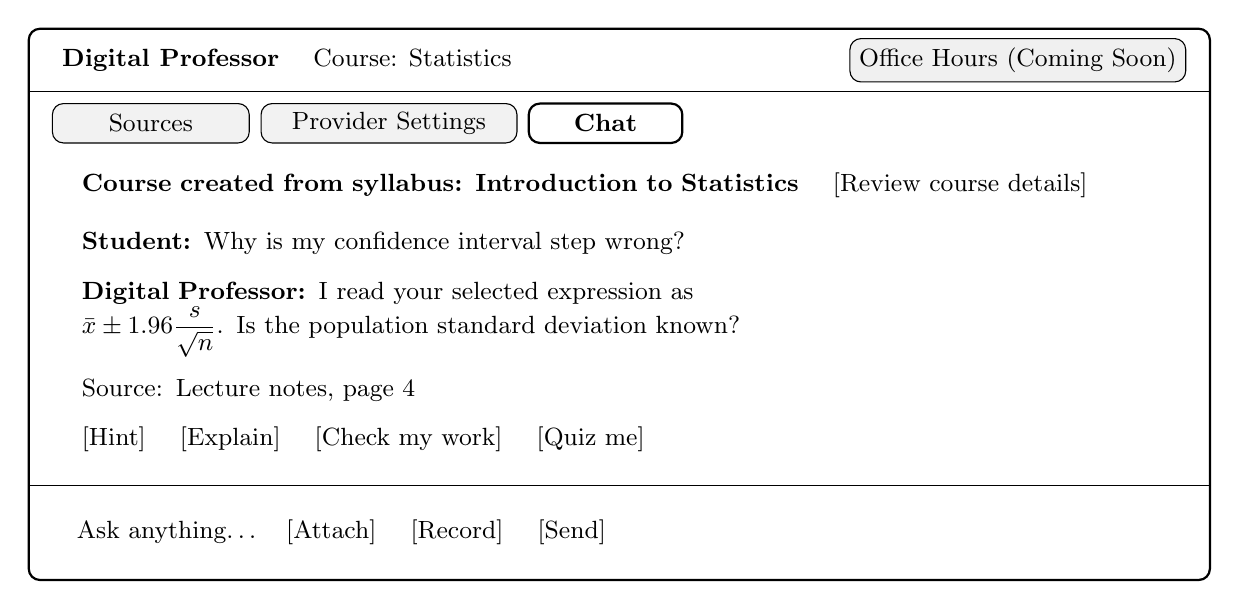
\begin{tikzpicture}[font=\small]
\draw[rounded corners,thick] (0,0) rectangle (15,7);
\node[anchor=west] at (0.3,6.6) {\textbf{Digital Professor} \quad Course: Statistics};
\node[anchor=east,draw,rounded corners,fill=gray!12] at (14.7,6.6) {Office Hours (Coming Soon)};
\draw (0,6.2) -- (15,6.2);
\draw[rounded corners,fill=gray!10] (0.3,5.55) rectangle (2.8,6.05);
\draw[rounded corners,fill=gray!10] (2.95,5.55) rectangle (6.2,6.05);
\draw[rounded corners,fill=white,thick] (6.35,5.55) rectangle (8.3,6.05);
\node at (1.55,5.8) {Sources};
\node at (4.575,5.8) {Provider Settings};
\node at (7.325,5.8) {\textbf{Chat}};
\node[anchor=north west,text width=13.8cm] at (0.55,5.3) {\textbf{Course created from syllabus: Introduction to Statistics} \quad [Review course details]\\[10pt]
\textbf{Student:} Why is my confidence interval step wrong?\\[7pt]
\textbf{Digital Professor:} I read your selected expression as\\
\(\displaystyle \bar{x}\pm1.96\frac{s}{\sqrt{n}}\). Is the population standard deviation known?\\[7pt]
Source: Lecture notes, page 4\\[7pt]
[Hint] \quad [Explain] \quad [Check my work] \quad [Quiz me]};
\draw (0,1.2) -- (15,1.2);
\node[anchor=west,text width=14cm] at (0.5,0.6) {Ask anything\ldots\quad [Attach] \quad [Record] \quad [Send]};
\end{tikzpicture}
\caption{Proposed tabbed interface with Chat active. Sources handles syllabus onboarding and later uploads; Provider Settings contains model and speech choices. \emph{Office Hours} remains marked \emph{Coming Soon}.}
\end{figure}

\subsection{Optional shared-work view inside the chat}
When a student opens a document, image, or handwritten artifact, the chat may temporarily display a larger shared-work view. All input modes refer to the same selected artifact. This view supplements the tabbed chatbot interface rather than replacing it.

\begin{figure}[htbp]
\centering
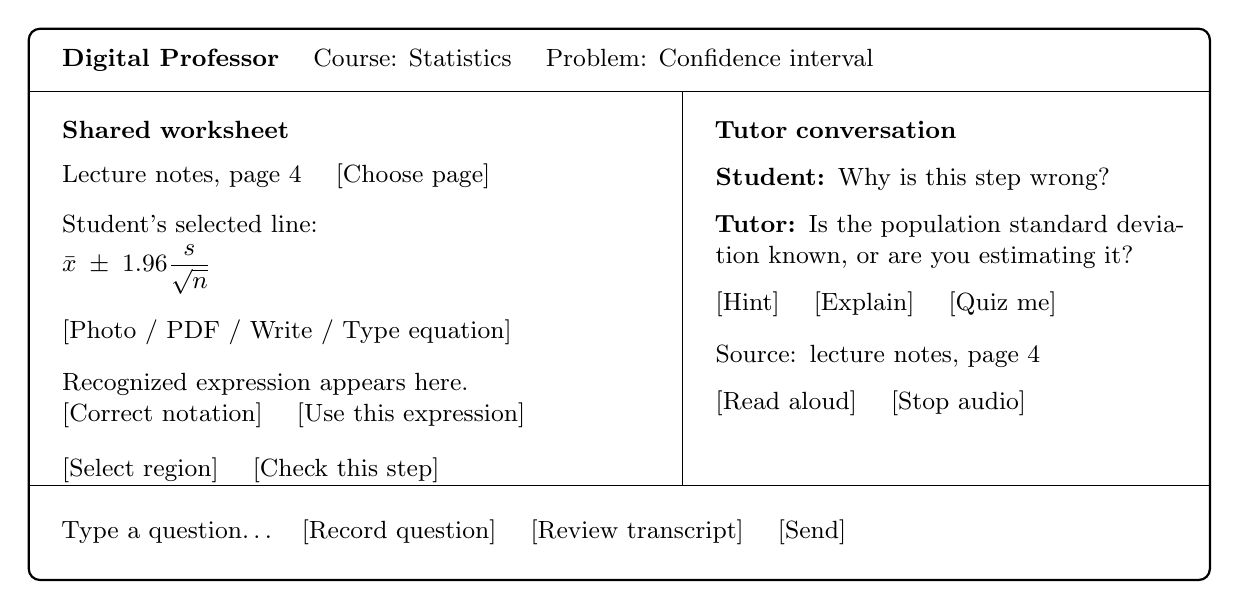
\begin{tikzpicture}[font=\small]
\draw[rounded corners,thick] (0,0) rectangle (15,7);
\node[anchor=west] at (0.3,6.6) {\textbf{Digital Professor} \quad Course: Statistics \quad Problem: Confidence interval};
\draw (0,6.2) -- (15,6.2);
\draw (8.3,1.2) -- (8.3,6.2);
\node[anchor=north west,text width=7.4cm] at (0.3,5.95) {\textbf{Shared worksheet}\\[5pt]
Lecture notes, page 4 \quad [Choose page]\\[7pt]
Student's selected line:\\[3pt]
\(\displaystyle \bar{x}\;\pm\;1.96\frac{s}{\sqrt{n}}\)\\[8pt]
[Photo / PDF / Write / Type equation]\\[8pt]
Recognized expression appears here.\\[0pt]
[Correct notation] \quad [Use this expression]\\[9pt]
[Select region] \quad [Check this step]};
\node[anchor=north west,text width=5.9cm] at (8.6,5.95) {\textbf{Tutor conversation}\\[6pt]
\textbf{Student:} Why is this step wrong?\\[6pt]
\textbf{Tutor:} Is the population standard deviation known, or are you estimating it?\\[6pt]
[Hint] \quad [Explain] \quad [Quiz me]\\[8pt]
Source: lecture notes, page 4\\[6pt]
[Read aloud] \quad [Stop audio]};
\draw (0,1.2) -- (15,1.2);
\node[anchor=west,text width=14cm] at (0.3,0.6) {Type a question\ldots\quad [Record question] \quad [Review transcript] \quad [Send]};
\end{tikzpicture}
\caption{Proposed tablet landscape or desktop view. On narrow screens, switch between worksheet and conversation while preserving the selection. Example dialogue is illustrative, not output from an evaluated system.}
\end{figure}

\textbf{Example student journey.}
\begin{enumerate}
\item Open the app and upload a syllabus when prompted in the Sources tab. Review the extracted course name and metadata, edit anything incorrect, and confirm creation of the course workspace.
\item Add notes, a homework PDF, and a photo or handwritten attempt in the Sources tab, then return to Chat.
\item Ask in chat, by text or recorded voice, ``Why is this confidence interval step wrong?'' The system infers that the student wants step-level feedback and determines which attached material is relevant.
\item The orchestrator calls document retrieval, image/OCR, transcription, or equation handling only when required. Ambiguous transcription or notation is shown to the student for correction.
\item For a small independent normal sample with unknown population standard deviation, discuss the appropriate Student's $t$ interval and its assumptions. The tutor links to the supplied course explanation rather than inventing a page citation.
\item The student revises the expression to $\bar{x}\pm t_{1-\alpha/2,n-1}s/\sqrt{n}$, explains the choice, and requests feedback. The tutor gives a follow-up question and saves a short progress note.
\end{enumerate}

The same interaction can discuss a free-body diagram or a written argument by changing course materials and evaluation criteria. This is the operational meaning of course-agnostic: reusable interaction and context handling, with domain-dependent correctness checks.

\textbf{Minimal conceptual flow:}
\begin{center}
\fbox{\parbox{0.92\textwidth}{\centering
Text / voice recording / selected page / image / ink\\
$\downarrow$\\
Capture and preview $\rightarrow$ optional transcription or OCR $\rightarrow$ student correction\\
$\downarrow$\\
Tutoring request + course evidence + current attempt\\
$\downarrow$\\
Generative model + optional bounded computation\\
$\downarrow$\\
Visible feedback, source links, equations, and optional spoken explanation}}
\end{center}
Keep these boundaries replaceable. A useful request record contains a session ID, course ID, question, inferred intent, attachment/page/region references, original input, corrected notation, active providers, and requested response format. Provider-specific adapters can change without rewriting the student's workflow.

\section{Initial architecture: one orchestrator with modality tools}
The first prototype should use a single tutoring orchestrator rather than a manager delegating to multiple autonomous agents. Document ingestion, equation rendering, tablet capture, OCR, transcription, and speech synthesis are mostly bounded processing tasks. Implement them as services or tools that return structured results. This retains modularity while avoiding extra model calls, prompts, latency, cost, and coordination failures.

\begin{center}
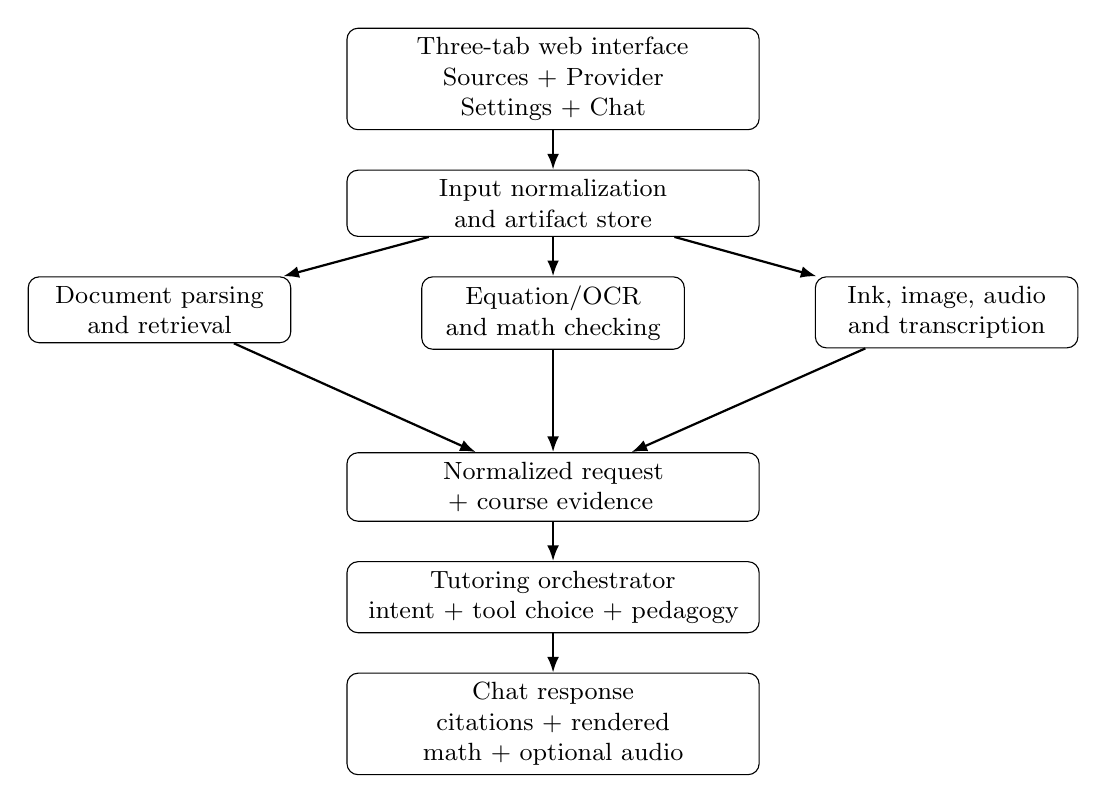
\begin{tikzpicture}[node distance=5mm and 7mm, font=\small,
box/.style={draw,rounded corners,align=center,minimum height=8mm,text width=3.1cm},
wide/.style={draw,rounded corners,align=center,minimum height=8mm,text width=5.0cm},
arr/.style={-{Latex[length=2mm]},thick}]
\node[wide] (ui) {Three-tab web interface\\Sources + Provider Settings + Chat};
\node[wide,below=of ui] (normal) {Input normalization and artifact store};
\node[box,below left=of normal] (doc) {Document parsing\\and retrieval};
\node[box,below=of normal] (math) {Equation/OCR\\and math checking};
\node[box,below right=of normal] (media) {Ink, image, audio\\and transcription};
\node[wide,below=13mm of math] (context) {Normalized request + course evidence};
\node[wide,below=of context] (tutor) {Tutoring orchestrator\\intent + tool choice + pedagogy};
\node[wide,below=of tutor] (response) {Chat response\\citations + rendered math + optional audio};
\draw[arr] (ui) -- (normal);
\draw[arr] (normal) -- (doc);
\draw[arr] (normal) -- (math);
\draw[arr] (normal) -- (media);
\draw[arr] (doc) -- (context);
\draw[arr] (math) -- (context);
\draw[arr] (media) -- (context);
\draw[arr] (context) -- (tutor);
\draw[arr] (tutor) -- (response);
\end{tikzpicture}
\end{center}

A modality service should return structured data rather than a conversational answer. A result can contain the input modality, original artifact ID, recognized text or LaTeX, confidence, provenance, and a \texttt{needs\_confirmation} flag. The tutoring orchestrator receives these results with course evidence, determines the student's intent, selects any further tools, and produces one coherent student-facing response.

\subsection{Path toward a manager--worker agent system}
The architecture should leave room to promote selected tools into reasoning workers. A later manager agent could understand the request, create a task plan, and delegate open-ended work to agents that independently retrieve evidence, solve a problem, inspect a diagram, critique a derivation, or design a Socratic response. Deterministic operations such as KaTeX rendering, file conversion, stroke capture, and basic transcription should remain services even in that design.

Expansion is justified when evaluation shows that complex requests benefit from independent reasoning, parallel work, or cross-checking. At that stage, the tutoring orchestrator becomes the manager and synthesizes worker outputs into one student-facing answer with source provenance. Until then, a one-orchestrator design is easier to evaluate because failures can be attributed to input processing, retrieval, reasoning, or response generation.

\subsection{Office Hours: a restricted future capability}
The interface includes an \emph{Office Hours} control to make the product direction concrete, but the initial prototype labels it \emph{Coming Soon} and does not depend on live audio or video. The intended experience simulates a student visiting a professor's office: the student brings a question or attempted solution, the professor diagnoses the point of confusion, works through one idea at a time, and checks whether the student is following before continuing.

This behavior should also govern ordinary chat. After each substantial explanation or reasoning step, the tutor explicitly checks comprehension with a short question such as ``Does that step make sense?'', ``What would you substitute next?'', or ``Can you explain why that assumption matters?'' The follow-up should match the situation: a simple check-in can preserve conversational flow, while a brief retrieval or application question provides stronger evidence of understanding. If the student is unsure, the tutor should rephrase, use a smaller example, or step back to the missing prerequisite instead of continuing the original explanation.

The first Office Hours implementation can be a synchronous text session or push-to-talk conversation with visible transcripts. Video input is intentionally deferred; it is not necessary to reproduce the core educational behavior of office hours. Synchronous voice can be enabled after the system demonstrates reliable source grounding, intent handling, interruption behavior, transcript quality, latency, cost controls, and session recovery. The eventual mode reuses the same Sources tab, provider configuration, artifact store, and tutoring policies rather than becoming a separate application.

\section{Prototype priorities and feasibility tests}
\begin{enumerate}
\item \textbf{First demonstrable slice:} the three-tab web interface, syllabus upload and confirmed course-name extraction, open-ended text dialogue, source management, provider configuration, one selected PDF page or photo, rendered and editable equations, and source-linked feedback. Demonstrate a full attempt--hint--revision loop in statistics and an engineering topic.
\item \textbf{Small extensions:} push-to-talk, optional TTS, and an explicit-submit stylus canvas. Each should fall back to the existing text/image path if recognition fails.
\item \textbf{Subsequent experiments:} corpus retrieval, long recordings, improved stroke recognition, and bounded symbolic/numerical checks. Add only the services needed by observed failures.
\item \textbf{Later research:} enable \emph{Office Hours} first as synchronous text or interruptible voice without video; evaluate manager--worker reasoning for complex requests; then consider optional visual input, native PencilKit recognition, and synchronized devices. Compare each addition's learning and usability benefit against its complexity.
\end{enumerate}

\textbf{Evaluation proposal, not reported results.} Assemble 30--50 representative prompts spanning statistics and engineering, with typed references and matched audio, photo, or ink variants. Include unclear inputs and questions not answered by the supplied material. Use consenting pilot participants and preserve only the data needed for the study.

\begin{itemize}
\item \textbf{Recognition:} measure transcript word error rate, but separately score critical words, signs, subscripts, and full-expression correctness. Record how often users must correct input and how long correction takes.
\item \textbf{Grounding and tutoring:} have a knowledgeable reviewer assess correctness, assumption checking, source support, hint usefulness, and whether feedback addresses the student's actual step. Score perception errors separately from reasoning errors.
\item \textbf{Responsiveness and reliability:} report median and 95th-percentile time from submission to useful feedback, time to first audio, upload failures, and recovery after network interruption. An initial target might be useful text feedback within five seconds for a short request; this is an engineering target to validate, not a provider guarantee.
\item \textbf{Cost:} log actual token, audio-duration, OCR-page, storage, and hosting usage per completed task. Compare total cost per successful tutoring interaction, including retries and corrections, rather than isolated model-call prices.
\item \textbf{Learning and usability:} compare text-only with added modalities on matched tasks, counterbalance order, and collect completion time, correction burden, preference, and a short transfer question. Report uncertainty and participant-level variation; a small convenience pilot supports feasibility findings, not broad learning-effect claims.
\end{itemize}

An integration is worth keeping when it reduces student effort or improves demonstrated feedback quality. Log model/version and input conditions so results remain interpretable as services change. Make recording explicit, retain text alternatives, and define deletion and course-access behavior before using real student work. Full autonomous grading, institutional integration, and replacing every professor responsibility remain outside this initial interaction demonstration.

\clearpage
\part{Related Notes}

\section{Training and tuning for mathematical capability}
The project may eventually adapt an open-weight language or vision-language model using existing mathematical datasets. This could improve mathematical notation, intermediate reasoning, tool use, or recognition of visually presented problems. It should follow a measured baseline using prompting, course-document retrieval, and external math tools. Fine-tuning is an optimization step, not a substitute for grounding, symbolic verification, or tutoring-policy design.

There are also two separate targets. \emph{Mathematical problem solving} concerns arriving at a correct solution. \emph{Mathematical tutoring} concerns diagnosing the student's current understanding, selecting an appropriate hint, asking a useful question, checking comprehension, and avoiding unnecessary answer disclosure. Most math datasets train or evaluate the first target. A Digital Professor will need additional tutoring dialogues and preference data for the second.

\subsection{Candidate datasets and intended use}
\begin{longtable}{@{}P{0.19\textwidth}P{0.27\textwidth}P{0.27\textwidth}P{0.19\textwidth}@{}}
\toprule
Dataset & Contents & Potential project use & Important note \\
\midrule
\endfirsthead
\toprule Dataset & Contents & Potential project use & Important note \\
\midrule
\endhead
\href{https://huggingface.co/collections/AI-MO/numinamath}{NuminaMath} \cite{numinamath} & A collection of competition-style math problems and generated solution traces, including chain-of-thought and tool-integrated-reasoning variants. & Supervised fine-tuning for written mathematical reasoning or tool-use formats. & Filter incorrect, duplicated, overly long, and style-inappropriate solutions; verify the specific release and license. \\
\addlinespace
\href{https://github.com/mathllm/MATH-V}{MATH-Vision (MATH-V)} \cite{mathvision} & 3,040 visual competition problems spanning multiple mathematical disciplines and difficulty levels. & Multimodal evaluation of diagrams, geometry, plots, and other visual context. & Prefer it as a held-out benchmark. Training on evaluation examples would invalidate comparison results. \\
\addlinespace
\href{https://github.com/hendrycks/math}{MATH} \cite{mathdataset} & Competition mathematics problems with step-by-step solutions in natural language and LaTeX. & Train on the official training split; evaluate mathematical reasoning by subject and difficulty. & Preserve test separation and check for overlap with derivative datasets. \\
\addlinespace
\href{https://huggingface.co/datasets/nvidia/OpenMathInstruct-2}{OpenMathInstruct-2} \cite{openmath} & Large-scale synthetic math instruction data with problem-solution pairs and released training resources. & Supervised fine-tuning of an open-weight base or instruction model. & Scale does not guarantee correctness; sample, verify, deduplicate, and filter before training. \\
\addlinespace
\href{https://huggingface.co/datasets/meta-math/MetaMathQA}{MetaMathQA} \cite{metamath} & Augmented mathematical questions and responses derived from common reasoning datasets. & Lower-cost experiment for mathematical instruction tuning and question reformulation. & Synthetic augmentation can repeat source patterns and model-specific errors. \\
\addlinespace
\href{https://github.com/openai/grade-school-math}{GSM8K} \cite{gsm8k} & Approximately 8,500 linguistically diverse grade-school word problems. & A small, interpretable baseline for arithmetic word-problem reasoning and verifier experiments. & Narrower and easier than the intended university statistics and engineering scope. \\
\addlinespace
\href{https://github.com/google-deepmind/mathematics_dataset}{DeepMind Mathematics Dataset} \cite{deepmindmath} & Generated school-level questions across arithmetic, algebra, calculus, measurement, probability, and related categories. & Controlled curriculum experiments, data generation, and stress tests with known answers. & Template-generated examples may not resemble authentic student misconceptions or course language. \\
\addlinespace
\href{https://github.com/HZQ950419/Math-LLaVA}{MathV360K / Math-LLaVA} \cite{mathllava} & Multimodal mathematical question-answer pairs collected and synthesized from multiple visual-math sources. & Candidate visual instruction-tuning data for an open vision-language model. & Audit licenses and provenance across constituent sources and hold out independent visual benchmarks. \\
\addlinespace
\href{https://github.com/lupantech/MathVista}{MathVista} \cite{mathvista} & A 6,141-example benchmark combining mathematical and visual reasoning tasks. & Evaluation across visual, scientific, statistical, algebraic, and geometric reasoning. & The official repository describes it as a test set and prohibits using it as training data. \\
\bottomrule
\end{longtable}

\subsection{Recommended tuning sequence}
\begin{enumerate}
\item \textbf{Establish an untuned baseline.} Evaluate a hosted or open-weight model on representative statistics and engineering questions, handwritten or visual inputs, course-grounded questions, and tutoring conversations. Record mathematical correctness and pedagogical quality separately.
\item \textbf{Build clean evaluation sets first.} Reserve MATH-Vision, MathVista, official test splits, and a private project set before assembling training data. Deduplicate semantically as well as by exact text because many datasets derive from MATH, GSM8K, competitions, or one another.
\item \textbf{Use supervised fine-tuning selectively.} Begin with a small, filtered mixture such as NuminaMath, OpenMathInstruct-2, MATH training data, or MetaMathQA. Normalize answer formats and retain provenance. Compare the tuned checkpoint against the same frozen baseline.
\item \textbf{Add verifier or tool-use behavior.} Train examples in which the model calls a constrained symbolic or numerical tool, checks units and assumptions, and reports when a result cannot be verified. Correct tool traces matter more than verbose reasoning text.
\item \textbf{Tune tutoring behavior separately.} Create or curate dialogues containing a student attempt, diagnosed misconception, next instructional move, comprehension check, and response to uncertainty. Use expert review or preference optimization so the model learns to teach rather than simply reveal solutions.
\item \textbf{Consider multimodal tuning only after text experiments.} Visual fine-tuning requires an appropriate vision-language base model, more memory, careful image preprocessing, and independent visual evaluation. MATH-Vision and MathVista should remain benchmarks; a training-oriented resource such as MathV360K is a more plausible starting point after its provenance is reviewed.
\end{enumerate}

\subsection{Practical risks and decision criteria}
Dataset licenses, terms, image rights, and model licenses must be reviewed for the exact versions used. Dataset cards can change, and a permissive code license does not automatically grant unrestricted rights to every underlying problem or image. Store the dataset version, source URL, license information, transformations, and split assignment in a data manifest.

Generated solution traces may be fluent but wrong. Before tuning, validate final answers where possible with symbolic or numerical tools and manually inspect samples across topics. Remove answer-only examples if the desired behavior is explanatory, and avoid training the model to expose long solutions when the tutoring policy calls for hints and comprehension checks.

Proceed with tuning only if it improves a defined failure mode enough to justify training and serving costs. Useful measures include exact or symbolic answer correctness, diagram-dependent accuracy, unit and assumption handling, source grounding, misconception diagnosis, hint quality, comprehension checking, latency, and cost per completed tutoring interaction. A stronger MATH score alone would not establish a better Digital Professor.

\begin{thebibliography}{99}
\small
\bibitem{text} OpenAI. \emph{Text generation}. \url{https://developers.openai.com/api/docs/guides/text}.
\bibitem{realtime} OpenAI. \emph{Realtime and audio}. \url{https://developers.openai.com/api/docs/guides/realtime}.
\bibitem{live} Google. \emph{Gemini Live API overview}. \url{https://ai.google.dev/gemini-api/docs/live-api}.
\bibitem{livekit} LiveKit. \emph{Agents documentation: Introduction}. \url{https://docs.livekit.io/agents/}.
\bibitem{recorder} Mozilla contributors. \emph{MediaRecorder}. \url{https://developer.mozilla.org/en-US/docs/Web/API/MediaRecorder}.
\bibitem{stt} OpenAI. \emph{File transcription}. \url{https://developers.openai.com/api/docs/guides/speech-to-text}.
\bibitem{tts} OpenAI. \emph{Text to speech}. \url{https://developers.openai.com/api/docs/guides/text-to-speech}.
\bibitem{whisper} SYSTRAN and contributors. \emph{faster-whisper}. \url{https://github.com/SYSTRAN/faster-whisper}.
\bibitem{webspeech} Mozilla contributors. \emph{Web Speech API}. \url{https://developer.mozilla.org/en-US/docs/Web/API/Web_Speech_API}.
\bibitem{pdfjs} Mozilla. \emph{PDF.js}. \url{https://mozilla.github.io/pdf.js/}.
\bibitem{files} OpenAI. \emph{File inputs}. \url{https://developers.openai.com/api/docs/guides/file-inputs}.
\bibitem{retrieval} OpenAI. \emph{File search}. \url{https://developers.openai.com/api/docs/guides/tools-file-search}.
\bibitem{docling} Docling contributors. \emph{Docling: document processing for generative AI}. \url{https://github.com/docling-project/docling}.
\bibitem{pointer} Mozilla contributors. \emph{Pointer events}. \url{https://developer.mozilla.org/en-US/docs/Web/API/Pointer_events}.
\bibitem{myscript} MyScript. \emph{iinkTS: Get started}, Interactive Ink 4.1 documentation. \url{https://developer.myscript.com/doc/interactive-ink/4.1/web/iinkts/get-started/}.
\bibitem{mathpix} Mathpix. \emph{Mathpix OCR API: Introduction}. \url{https://docs.mathpix.com/}.
\bibitem{mathlive} MathLive. \emph{Mathfield: Introduction}. \url{https://mathlive.io/mathfield/}.
\bibitem{katex} KaTeX. \emph{API}. \url{https://katex.org/docs/api}.
\bibitem{sympy} SymPy contributors. \emph{Parsing}. \url{https://docs.sympy.org/latest/modules/parsing.html}.
\bibitem{media} Mozilla contributors. \emph{MediaDevices: getUserMedia() method}. \url{https://developer.mozilla.org/en-US/docs/Web/API/MediaDevices/getUserMedia}.
\bibitem{vision} OpenAI. \emph{Images and vision}. \url{https://developers.openai.com/api/docs/guides/images-vision}.
\bibitem{pencil} Apple. \emph{PencilKit}. \url{https://developer.apple.com/documentation/pencilkit}.
\bibitem{video} Google. \emph{Video understanding}. \url{https://ai.google.dev/gemini-api/docs/video-understanding}.
\bibitem{autotutor} Graesser, A. C., VanLehn, K., Rose, C. P., Jordan, P. W., and Harter, D. (2001). \emph{Intelligent Tutoring Systems with Conversational Dialogue}. AI Magazine, 22(4), 39. \url{https://doi.org/10.1609/aimag.v22i4.1591}.
\bibitem{handwritingparadigm} Anthony, L., Yang, J., and Koedinger, K. R. (2012). \emph{A paradigm for handwriting-based intelligent tutors}. International Journal of Human--Computer Studies, 70(11), 866--887. \url{https://doi.org/10.1016/j.ijhcs.2012.04.003}.
\bibitem{handwritingimpact} de Morais, F., and Jaques, P. A. (2022). \emph{Does handwriting impact learning on math tutoring systems?} Informatics in Education, 21(1), 55--90. \url{https://doi.org/10.15388/infedu.2022.03}.
\bibitem{handwritingreview} Rodrigues, L., Pereira, F. D., Marinho, M., Macario, V., Bittencourt, I. I., Isotani, S., Dermeval, D., and Mello, R. (2024). \emph{Mathematics intelligent tutoring systems with handwritten input: A scoping review}. Education and Information Technologies, 29, 11183--11209. \url{https://doi.org/10.1007/s10639-023-12145-3}.
\bibitem{multimedia} Moreno, R., and Mayer, R. E. (2002). \emph{Verbal redundancy in multimedia learning: When reading helps listening}. Journal of Educational Psychology, 94(1), 156--163. \url{https://doi.org/10.1037/0022-0663.94.1.156}.
\bibitem{tutoreval} Maurya, K. K., et al. (2025). \emph{Unifying AI Tutor Evaluation: An Evaluation Taxonomy for Pedagogical Ability Assessment of LLM-Powered AI Tutors}. Proceedings of NAACL 2025. \url{https://aclanthology.org/2025.naacl-long.57/}.
\bibitem{sciencetutor} Liu, M., Wang, L., and Zhang, W. (2025). \emph{Is Your Multimodal Large Language Model a Good Science Tutor?} \url{https://arxiv.org/abs/2505.06418}.
\bibitem{stepwise} Wang, R., et al. (2024). \emph{Stepwise Verification and Remediation of Student Reasoning Errors with Large Language Model Tutors}. \url{https://arxiv.org/abs/2407.09136}.
\bibitem{numinamath} AI-MO. \emph{NuminaMath collection}. \url{https://huggingface.co/collections/AI-MO/numinamath}.
\bibitem{mathvision} Wang, K., Pan, J., Shi, W., Lu, Z., Ren, H., Zhou, A., Zhan, M., and Li, H. (2024). \emph{Measuring Multimodal Mathematical Reasoning with the MATH-Vision Dataset}. NeurIPS 2024 Datasets and Benchmarks Track. \url{https://github.com/mathllm/MATH-V}.
\bibitem{mathdataset} Hendrycks, D., Burns, C., Kadavath, S., Arora, A., Basart, S., Tang, E., Song, D., and Steinhardt, J. (2021). \emph{Measuring Mathematical Problem Solving With the MATH Dataset}. NeurIPS 2021. \url{https://github.com/hendrycks/math}.
\bibitem{openmath} Toshniwal, S., Du, W., Moshkov, I., Kisacanin, B., Ayrapetyan, A., and Gitman, I. (2024). \emph{OpenMathInstruct-2: Accelerating AI for Math with Massive Open-Source Instruction Data}. \url{https://huggingface.co/datasets/nvidia/OpenMathInstruct-2}.
\bibitem{metamath} Yu, L., et al. (2023). \emph{MetaMath: Bootstrap Your Own Mathematical Questions for Large Language Models}. \url{https://github.com/meta-math/MetaMath}.
\bibitem{gsm8k} Cobbe, K., Kosaraju, V., Bavarian, M., Chen, M., Jun, H., Kaiser, L., Plappert, M., Tworek, J., Hilton, J., Nakano, R., Hesse, C., and Schulman, J. (2021). \emph{Training Verifiers to Solve Math Word Problems}. \url{https://github.com/openai/grade-school-math}.
\bibitem{deepmindmath} Saxton, D., Grefenstette, E., Hill, F., and Kohli, P. (2019). \emph{Analysing Mathematical Reasoning Abilities of Neural Models}. \url{https://github.com/google-deepmind/mathematics_dataset}.
\bibitem{mathllava} Shi, W., et al. (2024). \emph{Math-LLaVA: Bootstrapping Mathematical Reasoning for Multimodal Large Language Models}. \url{https://github.com/HZQ950419/Math-LLaVA}.
\bibitem{mathvista} Lu, P., et al. (2024). \emph{MathVista: Evaluating Mathematical Reasoning of Foundation Models in Visual Contexts}. \url{https://github.com/lupantech/MathVista}.
\end{thebibliography}
\end{document}
